%--------------------------------------------------------------------------------------------
% MPAS-A Overview
%--------------------------------------------------------------------------------------------

\chapter{MPAS-Atmosphere Overview}
\label{chap:atmosphere_overview}

The Model for Prediction Across Scales -- Atmosphere (MPAS-A) is a
non-hydrostatic atmosphere model that is part of a family of
Earth-system component models collectively known as MPAS.  All MPAS
models have in common their use of centroidal Voronoi tessellations for
their horizontal meshes, which has motivated the development of a common
software framework that provides a high-level driver program and
infrastructure for providing parallel execution, input and output, and
other software infrastructure.

\section{Features}

Important features of MPAS-A include:

\begin{itemize}
\item Fully-compressible, non-hydrostatic dynamics
\item Split-explicit Runge-Kutta time integration
\item Exact conservation of dry-air mass and scalar mass
\item Positive-definite and monotonic transport options
\item Generalized terrain-following height coordinate
\item Support for unstructured variable-resolution (horizontal) mesh integrations for the sphere and Cartesian planes.
\end{itemize}

At present, MPAS-A includes parameterizations of physical processes
taken from the Weather Research and Forecasting (WRF) Model
\footnote{\url{http://www.wrf-model.org/}.}. Specifically, MPAS-A has
support for:

\begin{itemize}
\item Radiation: CAM and RRTMG long-wave and short-wave radiation schemes
\item Land-surface: NOAH land-surface model
\item Surface-layer: Monin-Obukhov and MYNN
\item Boundary-layer: YSU and MYNN PBL schemes
\item Convection: Kain-Fritsch Tiedtke, New Tiedtke, and Grell-Freitas convection parameterizations
\item Cloud microphysics: WSM6, Kessler, and Thompson schemes
\end{itemize}

\section{Model components}

MPAS-A is comprised of two main components: the model, which includes
atmospheric dynamics and physics; and an initialization component for
generating initial conditions for the atmospheric and land-surface state as well as update files for sea-surface
temperature and sea ice. Both components (model and initialization) are built as {\it cores}
within the MPAS software framework and make use of the same driver
program and software infrastructure.  However, each component is compiled as
a separate executable.

\begin{figure}[htb]
\begin{center}
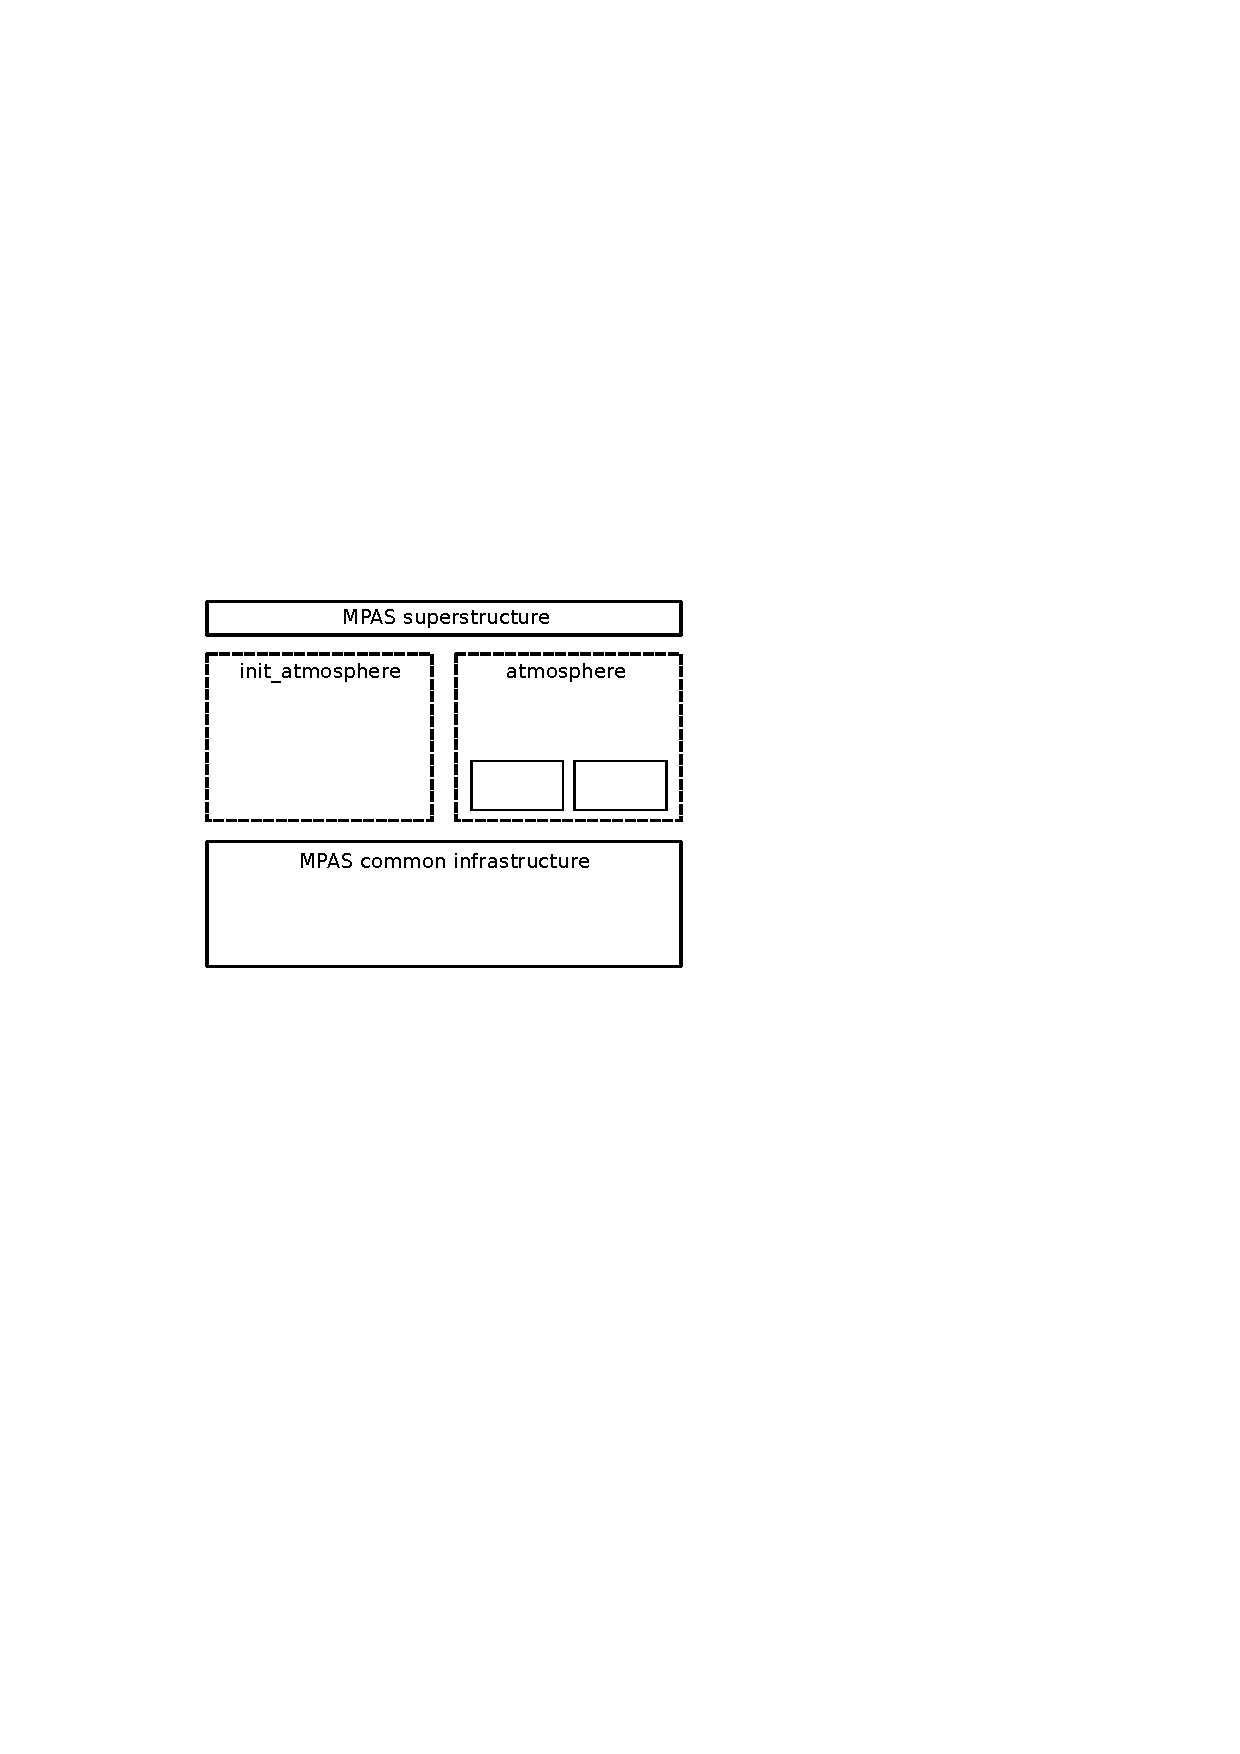
\includegraphics[width=3.5in]{figures/mpas-a_components.pdf}
\caption{The initialization and model components of MPAS-A are built as
separate {\em cores} within the MPAS framework.}
\label{fig:atm_components}
\end{center}
\end{figure}

A succinct description of building and running MPAS-A is given in Chapter \ref{chap:quick_start}, the Quick Start Guide.
Detailed instructions for building these components are given in Chapter
\ref{chap:mpas_build_instructions}, and the basic steps to create initial
conditions and run the MPAS-A model are outlined in Chapter
\ref{chap:running_mpas_a}.
